\documentclass[main.tex]{subfiles}
\usepgfplotslibrary{statistics}
\usepackage[group-separator={,}]{siunitx}
\begin{document}

\listoftodos

\section{Suboptimal
  approximations}\label{sec:suboptimal_approximations}
\todo[inline]{Update introduction here}
In this section we will look at a class of algorithms known as
\emph{lookahead policies}, that calculate the decisions on-line.
Whenever a decision must be made, these methods simulate the future
behaviour of the system and optimise the current decision based on
these simulations. First, we consider a special case called the
\emph{Certainty Equivalent Control} policy, which uses a point
estimate of the system (\citet[Ch.~6]{bertsekas2005dynamic}). For the
example system in this article, it turns out that we can solve
this approximate problem analytically.
Then, we investigate lookahead policies that take into account the
variability of the future system trajectories, which produce
results that are more similar to the optimal Bellman policy.
Numerical comparison experiments between the different policies are
made using the example pricing problem introduced in
\Cref{sec:bellman_example_markdown}.

\subsection{The Certainty Equivalent Control policy}
A popular, tractable, algorithm for solving stochastic optimal control
problems is the Certainty Equivalent Control (CEC) policy, as it is
named in \citet{bertsekas2005dynamic}.
It also known as (deterministic) Model
Predictive Control in the engineering community.
The algorithm is particularly practical, because the optimisation
problem is reduced to a standard deterministic problem that can
be solved with existing, commercial or open-source solvers which
handle very large systems.
At each decision time, a deterministic optimization problem for the
remaining decision horizon is solved. Only the decision for the
current time step is
used, whilst the subsequent decisions are discarded.
For each decision time $t=0,\dots,T-1$, the CEC algorithm for the pricing
problem calculates the current price using the following steps:
\begin{enumerate}
\item Observe state $s$.
\item Take a best estimate $w_{t+1},\dots,w_T$ of ${(W_\tau)}_{t+1}^T$.
\item Solve the optimization problem
  \begin{equation}
    \max_{\mathbf a\in A^{T-t}}\left\{\sum_{\tau=t}^{T-1}\mathbf
      a_\tau Q(S_\tau^{\mathbf a},\mathbf
      a_\tau,w_{\tau})-CS_T^{\mathbf a}\right\},
    \quad \text{s.t.}\quad S_t^{\mathbf a}=s.
  \end{equation}
\item Set the price corresponding to a maximizer
  $\mathbf a_t\in A$ above.
\end{enumerate}

For the one-product pricing problem, we can simplify the optimization
problem and in some cases obtain analytical solutions for the policy function.
First, let us consider the expected value estimate $w_\tau=\mathbb E
[W_\tau]=1$ for $\tau=t+1,\dots T$.
Then we can rewrite the maximisation problem to find
the certainty equivalent value function,
\begin{equation}
  \widetilde{v}(t,s)=
  \max_{\mathbf a\in A^{T-t}}\left\{\sum_{\tau=t}^{T-1}(\mathbf
    a_\tau+C)\min\left(s-\sum_{r=t}^{\tau-1}q(\mathbf a_r),q(\mathbf a_\tau)\right)-Cs\right\}.
  % \quad \text{s.t.}\quad \sum_{\tau=t}^{T-1}q(\mathbf a_t)\leq s.
\end{equation}
The optimal choice here is to let $\mathbf a_\tau=a^*\in A$ for each
$\tau$, such that the same amount of stock is forecast to be sold in
each period.
Then, $a^*=a^C(t,s)$ is given by the policy function
\begin{equation}
  a^C(t,s)=\argmax_{a\in A} \left\{(a+C)\min\left(
      \frac{s}{T-t},q(a)
    \right)\right\}.
  % ,\quad\text{s.t.}\quad q(a)\leq \frac{s}{T-t}.
\end{equation}
Let $\mathcal P_A$ be the projection operator from $\mathbb R$ onto the interval $A$.
Let us consider two families of demand functions that are
popular in the literature, see e.g.~\citet[Ch.~7]{talluri2006theory}.
If $q$ is of the form $a\mapsto q_1-q_2a$, with $q_1,q_2> 0$, then
the optimal policy $\alpha_t=a^C(t,S_t^\alpha)$ for the deterministic
problem is given by the function
\begin{equation}
  a^C(t,s)=\mathcal P_A \left[ \max\left(
      \frac{q_1}{q_2}-\frac{s}{q_2(T-t)},\frac{1}{2}\left(\frac{q_1}{q_2}-C
      \right) \right) \right].
\end{equation}
In the case when $q(a)=q_1e^{-q_2a}$, the policy function is
\begin{equation}\label{eq:cec_policy}
  a^C(t,s)=\mathcal P_A\left[
    \max\left( \frac{1}{q_2}\log\left( \frac{q_1(T-t)}{s}\right),
      \frac{1}{q_2}-C  \right)\right].
\end{equation}
The numerical experiments in the article are all made
with a demand function of the family $q(a)=q_1e^{-q_2a}$,  for a
single combination of the  system
parameters. We refer to the appendix for a
comparison between the Bellman policy and CEC policy for a larger
range of parameters.

\todo[inline]{Can we get error bounds comparing $\widetilde{v}$ and
  $v$? Maybe using ideas from \citet{bertsekas2005survey}
  If so, write out explicit expression for $\widetilde{v}$}
% We know that $\widetilde{v}(T,s)=v(T,s)$, and that by
% Jensen's inequality, $v(T-1,s)\leq \widetilde{v}(T-1,s)$.
% Does this bound hold for $t<T-1$ as well? I'm struggling to prove it
% \begin{align}
%   \widetilde{v}(t,s)
%   &=
%     \begin{cases}
%       s& \frac{s}{T-t}\leq \frac{q_1}{e^{q_2}}\\
%       \frac{1}{q_2}(\log(q_1(T-t))s-s\log s)&
%       \frac{q_1}{e^{-q_2}}<\frac{s}{T-t}\leq
%       \frac{q_1e^{{(\frac{1}{q_2}-C)}^+}}{e^{-q_2}}\\
%       \frac{q_1(T-t)}{e^{-q_2}}\left( {[\frac{1}{q_2}-C]}^++C \right)
%       e^{{(\frac{1}{q_2}-C)}^+}-Cs&\text{otherwise}
%     \end{cases}
% \end{align}
% \todo[inline]{Is $\widetilde{v}$ concave in $s$? I think we need to
%   require $q_2\geq 1$ and maybe that $C$ only takes certain values}

\subsubsection{Example system}\label{sec:cec_comparison_example}
\begin{figure}[htbp]
  \centering
  \begin{tikzpicture}
    \begin{axis}[
      xlabel={$s$},
      ylabel={Function value},
      title={Policy functions},
      legend cell align=left,
      ]
      \addplot[mark=none] table[x index = 0,y expr={\thisrowno{5}},col sep=comma]
      {./data/markdown_bellman_det_val_policy.csv};
      \addlegendentry{$a^B(t,s)$};
      \addplot[mark=none,dashed] table[x index = 0,y expr={\thisrowno{8}},col sep=comma]
      {./data/markdown_bellman_det_val_policy.csv};
      \addlegendentry{$a^C(t,s)$};
      \addplot[mark=none] table[x index = 0,y expr={\thisrowno{6}},col sep=comma]
      {./data/markdown_bellman_det_val_policy.csv};
      \addplot[mark=none,dashed] table[x index = 0,y expr={\thisrowno{9}},col sep=comma]
      {./data/markdown_bellman_det_val_policy.csv};
      \addplot[mark=none] table[x index = 0,y expr={\thisrowno{7}},col sep=comma]
      {./data/markdown_bellman_det_val_policy.csv};
      \addplot[mark=none,dashed] table[x index = 0,y expr={\thisrowno{10}},col sep=comma]
      {./data/markdown_bellman_det_val_policy.csv};
      \draw (axis cs:0.45,0.55) node[anchor=north east] {$t=2$};
      \draw (axis cs:0.72,0.65) node[anchor=north east] {$t=1$};
      \draw (axis cs:0.75,0.75) node[anchor=south west] {$t=0$};
    \end{axis}
  \end{tikzpicture}

  % \vspace{1em}
  % \begin{tikzpicture}
  %   \begin{axis}[
  %     xlabel={$s$},
  %     ylabel={$[a^B(t,s)-a^C(t,s)]/a^B(t,s)$},
  %     title={\hspace{1em}Relative function difference},
  %     legend cell align=left,
  %     ]
  %     \addplot+[mark=none] table[x index = 0,y expr={1-\thisrowno{8}/\thisrowno{5}},col sep=comma]
  %     {./data/markdown_bellman_det_val_policy.csv};
  %     \addlegendentry{$t=0$};
  %     \addplot+[mark=none] table[x index = 0,y expr={1-\thisrowno{9}/\thisrowno{6}},col sep=comma]
  %     {./data/markdown_bellman_det_val_policy.csv};
  %     \addlegendentry{$t=1$};
  %     \addplot+[mark=none] table[x index = 0,y expr={1-\thisrowno{10}/\thisrowno{7}},col sep=comma]
  %     {./data/markdown_bellman_det_val_policy.csv};
  %     \addlegendentry{$t=2$};
  %   \end{axis}
  % \end{tikzpicture}
  % \todo[inline]{Remove the relative difference comparison?}
  \caption{Comparison of the CEC and Bellman policy functions $a^C$ and
    $a^B$.
    The CEC function sets
    higher prices than the Bellman function for large $s$.
    % Observe the spikes in the difference plot for $t<T-1$:
    % In a small interval, $a^B(t,s)\geq a^C(t,s)$, before both functions
    % reach the boundary price $a_{\mathrm{max}}=1$. This sudden, relative increase in
    % the Bellman function compared to $a^C$ is due to the
    % diffusion of the value function caused by the
    % random variables $W_t$.
  }\label{fig:bellman_det_policy_difference}
\end{figure}

The example system in \Cref{sec:bellman_example_markdown} has a demand
function of the form $q(a)=q_1e^{-q_2a}$, where $q_1=e^2/3$ and
$q_2=3$. We can therefore compare the optimal Bellman policy with the
pricing policy that a CEC algorithm would create.
Denote the Bellman policy function by $a^B$, and consider
$a^B(t,s)-a^C(t,s)$ for each $t=0,\dots,T-1$. The plot in
\Cref{fig:bellman_det_policy_difference} shows this difference.
Both of the policy functions reach the upper bound in $A$ for small values
of $s$, but most of the time, the Bellman policy is pricing the products
lower than the CEC policy.

What is more important than how the policy function works, is how it
impacts the goal of the decision-process. Thus, we would like to see
how the two policy processes $\alpha^B$ and $\alpha^C$ perform.
One way to evaluate their performance is to look at
the distribution of the profits $P^{\alpha^B}$ and $P^{\alpha^C}$.
We remind the reader that
$P^\alpha =
\sum_{t=0}^{T-1}\alpha_tQ(S_t^\alpha,\alpha_t,W_{t+1})-CS_T^\alpha$.
From the opitimality of the Bellman policy function, we should have
that $\mathbb E_W[P^{\alpha^B}]\geq \mathbb E_W[P^{\alpha^C}]$.
However, marginalising a random variable with the expectation operator
loses a lot of information which can be of interest.
An approximation of the distributions of $P^{\alpha^B}, P^{\alpha^C}$
and their difference
$P^{\alpha^B}-P^{\alpha^C}$, based on \num{10000} realisations of the
underlying $W$, can be seen in \Cref{fig:bellman_det_vals}.
Indeed in the experiment, the average value of following the
Bellman policy is higher than following the CEC policy.
However, from the bottom figure we see that
in more than half of the cases, the CEC policy outperforms the optimal
policy $\alpha^B$. What we can take from this experiment is that
the CEC policy induces a more risk-seeking pricing strategy than
$\alpha^B$: It results in slightly larger profits for a majority of the
realisations of $W$, but at a cost of taking a more significant
reduction in
profits in the remaining realisations.
\begin{figure}[p]
  \centering
  \begin{tikzpicture}[scale=0.8]
    \begin{axis}[
      xlabel=$P^{\alpha^B}$,
      ylabel=Count,
      title={Simulations of Bellman policy},
      xmin=0.565, xmax=0.695,
      ymax=2000,
      ]
      \addplot[blue,hist={bins=30}] table [y index = 0,col sep=comma]
      {./data/markdown_bellman_det_vals.csv};
    \end{axis}
  \end{tikzpicture}%
  \begin{tikzpicture}[scale=0.8]
    \begin{axis}[
      xlabel=$P^{\alpha^C}$,
      title={Simulations of CEC policy},
      xmin=0.565, xmax=0.695,
      ymax=2000,
      ]
      \addplot[blue,hist={bins=30}] table [y index = 1,col sep=comma]
      {./data/markdown_bellman_det_vals.csv};
      \draw[<-] (axis cs:0.62,220) --
      (axis cs:0.605,600) node[anchor=south] {Fatter lower tail};
    \end{axis}
  \end{tikzpicture}

  \vspace{1em}
  \begin{tikzpicture}
    \begin{axis}[
      xlabel=$P^{\alpha^B}-P^{\alpha^C}$,
      ylabel=Count,
      title={Simulations of Bellman and CEC policies},
      ]
      \addplot[red,hist={bins=30}] table [y expr = {(\thisrowno{0}-\thisrowno{1})},col sep=comma]
      {./data/markdown_bellman_det_vals.csv};
      \draw[dashed] (axis cs:0,-30) -- (axis cs:0,6000);
      \draw[<-] (axis cs:0.017,1000) -- (axis cs:0.015,2000)
      node[anchor=south] {$\alpha^B$ best};
      \draw[<-] (axis cs:-0.003,4000) -- (axis cs:0.005,4000) node[anchor=west] {$\alpha^C$ best};
    \end{axis}
  \end{tikzpicture}
  \todo[inline]{Show relative difference
    $(P^{\alpha^B}-P^{\alpha^C})/P^{\alpha^B}$ instead?}
  \caption{This shows the distributions from \num{10000} samples of
    the profits of following the Bellman and CEC policies.
    The sample mean $\mathbb E_W[P^{\alpha^B}-P^{\alpha^C}]\approx 3.8\times
    10^{-3}$, confirms that Bellman is better on average, as it should be.
    Importantly, however, in more than half the samples the suboptimal policy
    outperforms the Bellman policy.
  }\label{fig:bellman_det_vals}
\end{figure}

\todo[inline]{Add OLFC section here with table similar to \Cref{tbl:paramcomparisons}?}

\subsection{Bellman and CEC parameter comparisons}\label{sec:parameter_comparison}
In the previous sections, our numerical experiments have only shown
results for a fixed combination of the five parameters
termination time $T$, unsold items cost $C$, uncertainty $\gamma$, and
demand function parameters $q_1,q_2$.
In this section we explore the differences between the Bellman policy
and the CEC policy for a larger parameter range.
The formula for $a^C$ in \Cref{eq:cec_policy} indicates that the
initial price is largely determined by the relationship between
$Tq_1$ and $q_2$, and hence we choose to keep $T=3$ fixed whilst
varying $q_1$ and $q_2$.
We are interested in the difference between the profit following
a Bellman policy $\alpha^B$ and a CEC policy $\alpha^C$.
The policy $\alpha^B$ is computed numerically, and
$\alpha^C$ is obtained using the function $a^C$ from
the formula in \Cref{eq:cec_policy}.

\todo[inline]{Move table to here?}
In particular, the difference between the two policies is measured
using the $L^2$-norm with respect to the probability distribution
induced by the disturbance $(W_1,W_2,\dots,W_T)$, that is
\begin{equation}
  \left\|P^{\alpha^B}-P^{\alpha^C}\right\|_2
  =\sqrt{\mathbb E_W\left[{( P^{\alpha^B}-P^{\alpha^C} )}^2 \right]}.
\end{equation}

To reduce the number of combinations of parameters, we make the
simplification to choose only
four combinations of
$(C,\gamma)\in\{0.5,1\}\times\{0.05,0.1\}$.
Then,
for each combination of $(C,\gamma)$,
we can create a heatmap of the difference between the two policy
functions by varying the parameters $q_1,q_2$.
The relative $L^2$ difference between the CEC and Bellman policy outcomes
is shown in \Cref{fig:profit_diff_heatmaps}. The norms were approximated
with $1000$ samples from $(W_1,W_2,\dots,W_T)$.
Comparing the left and right column, we see that the relative difference doubles as
the standard deviation $\gamma$ is doubled. The cost $C$ plays a large
role, both in terms of the shape of the difference surface and its
magnitude.
The black region at the bottom right of the plots correspond to popular,
low-elasticity products where both policies choose to sell at the
maximum price $a=1$.
\begin{figure}[htbp]
  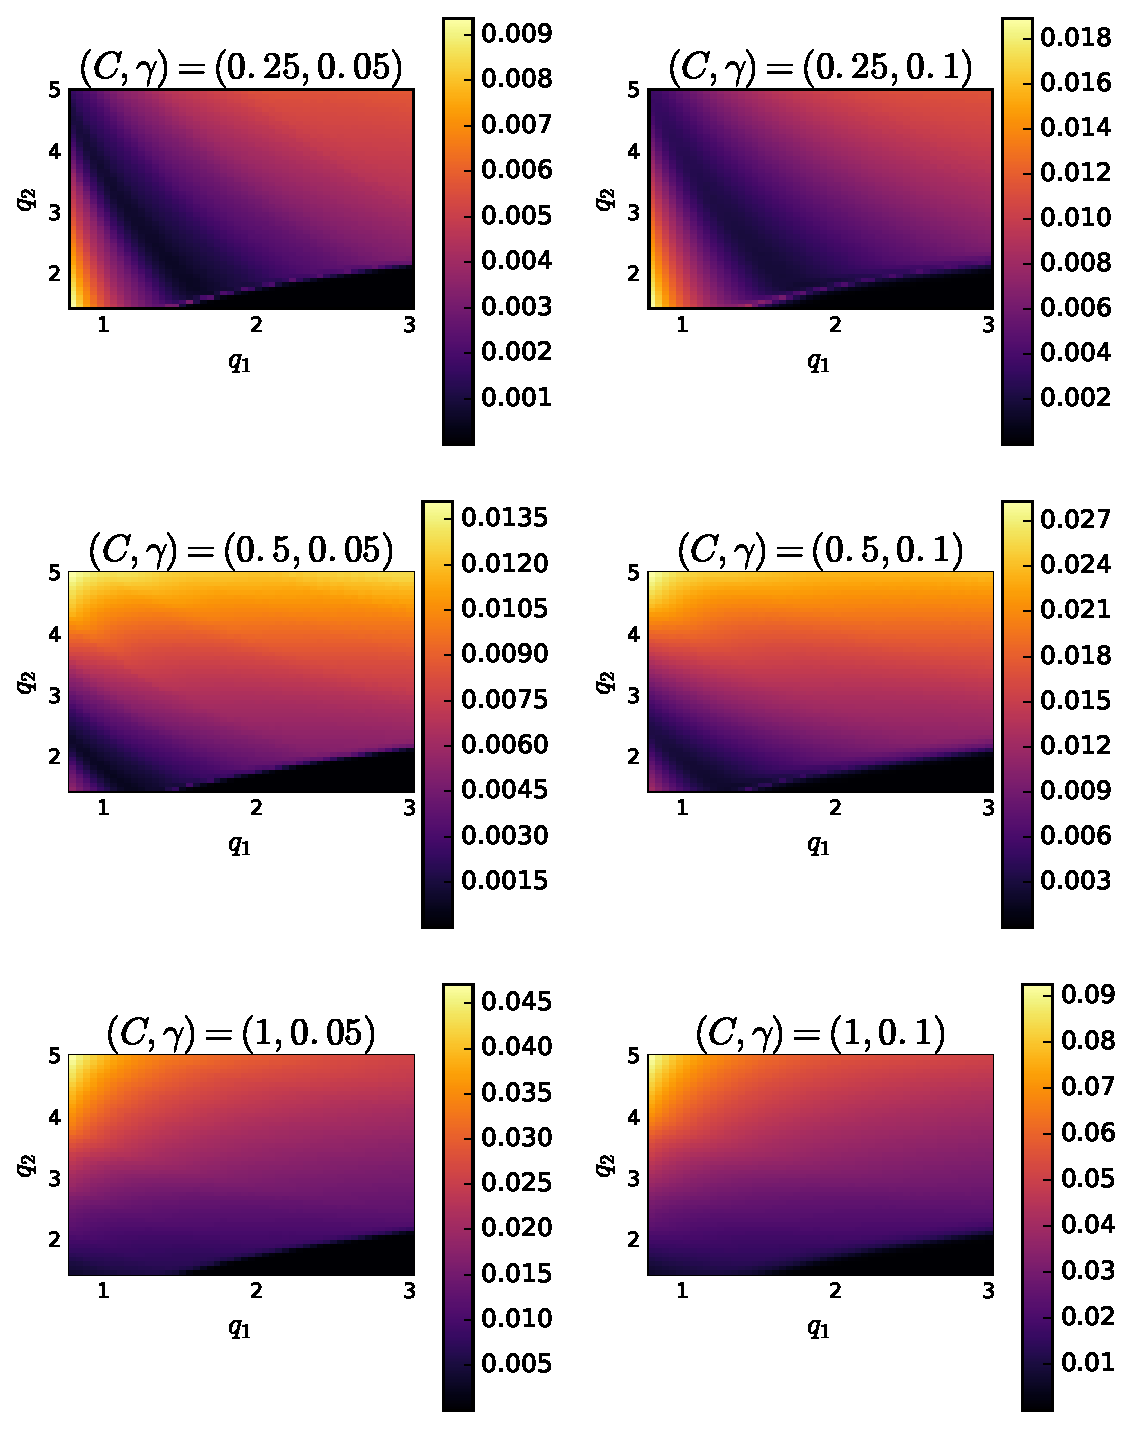
\includegraphics[width=\textwidth]{./img/profit_diff_heatmaps}
  \caption{The relative $L^2$ difference
    $\|P^{\alpha^B}-P^{\alpha^C}\|_2/\|P^{\alpha^B}\|_2$ representing
    how different the CEC policy is to the optimal Bellman policy.
    Each plot defines a combination of $(C,\gamma)$, whilst
    the axes vary the parameters $q_1,q_2$ of the demand function
    $q(a)=q_1e^{-q_2a}$.
    The white dot on the bottom, left plot corresponds to the
    parameters chosen for the experiments in this article.
  }\label{fig:profit_diff_heatmaps}
\end{figure}

The parameters chosen in this article's numerical experiments
are $C=1,\gamma=0.05,q_1=e^2/3\approx2.5,q_2=3$. This point lies
in the region where the relative difference is around $0.016$ --- see the
white dot in the
bottom, left subfigure in \Cref{fig:profit_diff_heatmaps}.
This difference is in the middle of that seen for all the
combinations of parameters, so the conclusions made in the article
should be considered as relevant for a wider range of systems.
\Cref{tbl:paramcomparisons} provides further data to underscore
the claim that the CEC policy
outperforms the Bellman policy the
majority of events, at the expense of a stronger underperformance
for the remainder of the events. Notably, the CEC policy is better
more than 50\% of the time for all the parameter
combinations considered in this article. The values in
\Cref{tbl:paramcomparisons} were approximated using $10,000$ samples
from $W$, and their corresponding parameter combinations are shown as
grey dots in \Cref{fig:profit_diff_heatmaps}.

\begin{table}[htbp]
  \centering
  \begin{tabular}{llllcccc}
    $C$ & $\gamma$ & $q_1$ & $q_2$ & $\mathcal Q_{0.05}$
    &Median & $\mathcal Q_{0.95}$ &$L_2$\\
    \toprule
    $0.25$ & $0.05$ & $2.0$ & $4.0$  & \textbf{-0.4} & \textbf{-0.3} & \textbf{0.6} & \textbf{0.4}\\
    $0.25$ & $0.1$ & $1.33$ & $2.67$ & \textbf{-0.5} & \textbf{-0.0} & \textbf{0.6} & \textbf{0.3}\\
    $0.5$ & $0.05$ & $2.67$ & $4.0$  & \textbf{-0.6} & \textbf{-0.6} & \textbf{1.9} & \textbf{1.1}\\
    $0.5$ & $0.1$ & $2.0$ & $2.67$   & \textbf{-0.9} & \textbf{-0.6} & \textbf{1.9} & \textbf{1.2}\\
    $1.0$ & $0.05$ & $1.33$ & $4.0$  & \textbf{-1.2} & \textbf{-1.1} & \textbf{5.3} & \textbf{2.7}\\
    $1.0$ & $0.1$ & $2.67$ & $2.67$  & \textbf{-1.5} & \textbf{-1.3} & \textbf{5.8} & \textbf{2.9}\\
    &&&&$\times 10^{-2}$&$\times 10^{-2}$&$\times 10^{-2}$&$\times 10^{-2}$\\
    \bottomrule
  \end{tabular}
  \caption{Statistics comparing $P^{\alpha^B}$ and $P^{\alpha^C}$ for six different
    parameter combinations. The columns $\mathcal Q_s$ represent the
    the $s^{\text{th}}$ quantile of the relative
    difference
    $1-P^{\alpha^C}/P^{\alpha^B}$. %Median is the same as $\mathcal Q_{0.5}$.
    The values in the column $L_2$ refers to the relative $L_2$
    difference $\|P^{\alpha^B}-P^{\alpha^C}\|_2/\|P^{\alpha^B}\|_2$
    from \Cref{fig:profit_diff_heatmaps}. Each of the parameter
    combinations correspond to a grey dot in \Cref{fig:profit_diff_heatmaps}.
  }\label{tbl:paramcomparisons}
\end{table}
\biblio
\end{document}

%%% Local Variables:
%%% mode: latex
%%% TeX-master: t
%%% TeX-command-extra-options: "-shell-escape"
%%% End:
